%! TEX Program = pdflatex

\documentclass{article}
\usepackage[a4paper,margin=1cm,left=2cm,right=2cm]{geometry}
\usepackage{newtxtext}
\usepackage{graphicx}
\usepackage{url}
\usepackage[colorlinks, urlcolor=blue]{hyperref}
\title{\huge Coefficient of Viscosity}
\author{Teddy van Jerry}
\date{\today}
\pagenumbering{gobble}
\renewcommand{\ttdefault}{pcr}

\begin{document}
    \maketitle

    Data in the experiment is dealt with \texttt{Param.py} which calculates the average speed $\overline{v}$, standard deviation, coefficient of viscosity $\eta$, Reynolds number $Re$ and the value after amending $\eta_1$ (if needed).

    Figure~\ref{fig:plot} below are drawn using \texttt{MATLAB 2021a}.

    The \texttt{MATLAB} and \texttt{Python} code is open source on GitHub under the MIT License: \url{https://github.com/Teddy-van-Jerry/SEU_Physics_Experiment}, \texttt{Coefficient of Viscosity}.

    It has helped some of my classmates in drawing an elegant figure.

    \begin{figure}[htbp]
        \centering
        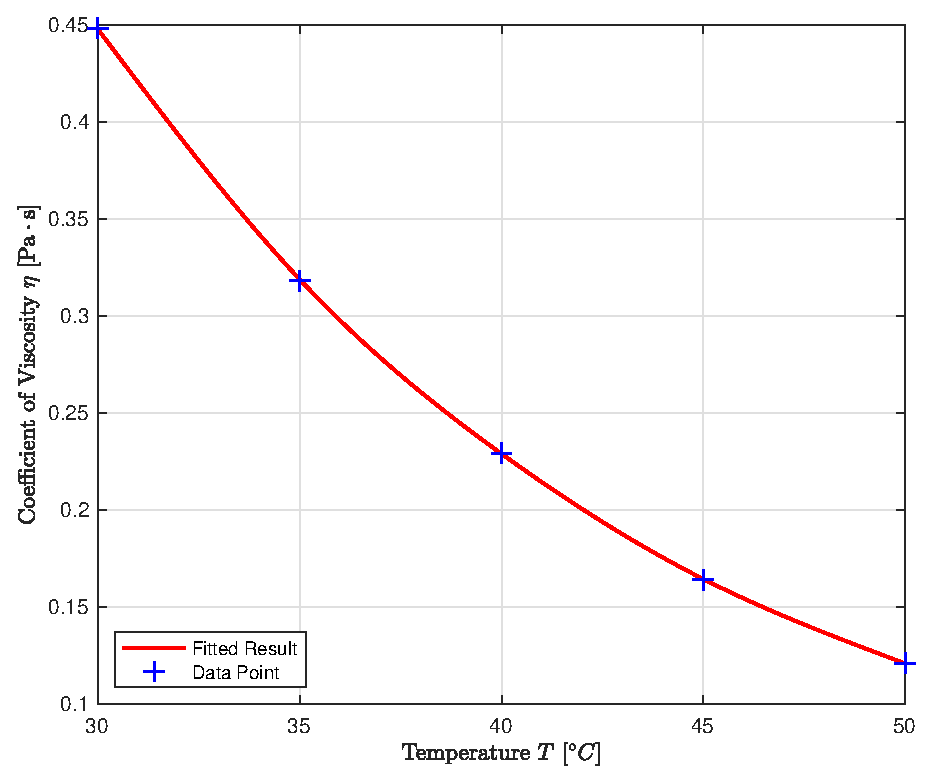
\includegraphics[width=.75\linewidth]{Plot.eps}
        \caption{$\eta$ vs. $T$}
        \label{fig:plot}
    \end{figure}
\end{document}

% ALL RIGHTS RESERVED (C) Teddy van Jerry
